% M0032
\title{Аналітична модель ініціювання відгалуження V-подібної міжфазної тріщини зсуву з її кутової точки}

% M0034
\author[1]{А.~О.~Камінський}
\author[1]{М.~Ф.~Селіванов\thanks{Автор для листування, \href{mailto:mfs@ukr.net}{mfs@ukr.net}.}}
\author[1,2]{М.~В.~Дудик}
\author[2]{Т.~В.~Поліщук}

% M0039
\affil[1]{Інститут механіки ім. С.~П.~Тимошенка НАН України, Київ, Україна}
\affil[2]{Уманський національний університет, Умань, Україна}

% M0042
\newcommand{\UAabstract}{В умовах плоскої деформації досліджено ініціювання відгалуження V-подібної міжфазної тріщини зсуву в кутовій точці ламаної межі поділу двох ізотропних пружних матеріалів. Тріщину розглянуто як заданий стаціонарний дефект із двома симетричними гілками, береги яких контактують без тертя. Сингулярне поле біля кутової точки тріщини використано як зовнішнє поле для малої розтягувальної зони передруйнування, орієнтованої вздовж бісектриси одного з матеріалів. Установлено умови, за яких стискальний контакт берегів міжфазної тріщини може поєднуватися з розтягувальним полем нормальних напружень у матеріалі, що містить зону передруйнування. За допомогою перетворення Мелліна, зрощування асимптотик, методу Вінера--Гопфа й умови регулярності напружень у вершині зони отримано замкнені аналітичні співвідношення для рівноважної довжини зони, її розкриття, роботи сил опору відриву та відповідного енергетичного параметра. Досліджено залежність цих характеристик від кута межі поділу, пружного контрасту та рівня навантаження. Показано, що утворення зони передруйнування послаблює сингулярність початкової конфігурації з V-подібною міжфазною тріщиною, хоча й не усуває її повністю. За фіксованої геометрії енергетична й деформаційна характеристики зони однозначно пов’язані, тому відповідні критерії ініціювання відгалуження еквівалентні за узгодженого вибору критичних параметрів матеріалу. Результати дають змогу прогнозувати ініціювання відгалуженої тріщини, якщо відповідну характеристику тріщиностійкості матеріалу задано незалежно.}

% M0044
\newcommand{\UAkeywords}{кусково-однорідне тіло, ламана межа поділу, V-подібна міжфазна тріщина зсуву, зона передруйнування, ініціювання відгалуження, метод Вінера--Гопфа}

% M0046
\maketitle
\begin{abstract}\UAabstract\end{abstract}
\noindent\textbf{Ключові слова.} \UAkeywords\par\medskip

% M0048
\section{Вступ}
% M0049
\label{sec:introduction}

% M0051
Кутові точки та злами меж поділу різнорідних матеріалів трапляються в багатьох клейових і багатоматеріальних з’єднаннях. У таких конфігураціях сама геометрія межі поділу може спричиняти локальну концентрацію напружень, яка істотно впливає на зародження пошкоджень~\citep{GacoinEtAl2009}. В ідеалізованій пружній постановці кутову точку межі поділу двох матеріалів описує степеневе власне поле, показник і кутова структура якого залежать від геометрії та пружного контрасту. Класичні умови існування та характеристики таких сингулярностей установлено для з’єднаних ізотропних клинів~\citep{BogyWang1971,DempseySinclair1981}. У подальших дослідженнях показано, що зміна кута може істотно змінювати як показник сингулярності, так і інтенсивність локального поля~\citep{MohammedLiechti2001}. Продовжують розвиватися методи визначення параметрів сингулярного поля в складніших тривимірних конфігураціях~\citep{MiyazakiFukudaNoda2025}. Запропоновано також маломасштабні співвідношення між параметрами поля непошкодженої кутової точки й параметрами короткої тріщини, що виходить із кутової точки межі поділу~\citep{LyuZhangMai2026}. Отже, характер руйнування залежить і від самої кутової сингулярності, і від її взаємодії з локальною нелінійною зоною або зоною передруйнування.

% M0069
Для початково непошкоджених кутових точок межі поділу двох матеріалів перехід від пружної сингулярності до локального руйнування досліджували як за параметрами асимптотичного поля, так і за допомогою моделей зі скінченною когезійною зоною або зоною передруйнування. Мохаммед і Ліхті поєднали експериментальні вимірювання з моделюванням зародження тріщини методом когезійної зони для різних кутів з’єднання двох матеріалів~\citeyearpar{MohammedLiechti2000}, а Лабосьєр і Данн дослідили ініціювання руйнування в тривимірних кутових точках межі поділу~\citeyearpar{LabossiereDunn2001}. Акісанья і Менґ показали, що застосування критичного параметра пружного поля кутової точки потребує достатнього розділення масштабів нелінійної зони й області, де переважає асимптотичне поле~\citeyearpar{AkisanyaMeng2003}. У сучасних когезійних моделях цю саму вимогу виражають через відношення характерної довжини зони руйнування до геометричного масштабу задачі~\citep{GormanThouless2022,ThoulessGoutianos2023}. У локальних аналітичних моделях ця вимога обґрунтовує маломасштабне припущення, за яким зона передруйнування мала порівняно з масштабом зовнішнього сингулярного поля, з яким її зрощують.

% M0086
Інша група досліджень стосується наявних міжфазних тріщин та їх можливого відхилення від межі поділу. Для ідеально крихкого руйнування класичні енергетичні дослідження встановили умови початкового відхилення тріщини від межі поділу~\citep{HeHutchinson1989}. Відповідні співвідношення для коефіцієнтів інтенсивності напружень і швидкостей вивільнення енергії отримано для тіл із двох анізотропних матеріалів~\citep{Wang1994}. Когезійні моделі показують, що вибір траєкторії може залежати від тріщиностійкості, когезійної міцності й характерного масштабу зони руйнування~\citep{ParmigianiThouless2006}. Аналітичні моделі малих зон передруйнування поблизу міжфазних тріщин дають змогу визначити довжину, розкриття й енергетичні характеристики зони~\citep{KaminskyEtAl2023}. Урахування несингулярного $T$-напруження показує також, що члени вищих порядків зовнішнього поля можуть давати помітні кількісні поправки~\citep{KaminskyDudykChornoivan2026}. Ці результати становлять методичну основу застосованого тут підходу із зоною передруйнування, хоча в цій роботі розглянуто іншу геометрію.

% M0102
Для кутових точок ламаних меж поділу аналітичні моделі зон передруйнування й тріщин розроблено в кількох близьких постановках. Дудик і Діхтяренко дослідили початкову стадію відхилення міжфазної тріщини з кутової точки~\citeyearpar{DudykDikhtyarenko2012}, а Камінський, Кіпніс і Поліщук розглянули початкову зону передруйнування, що виникає безпосередньо в кутовій точці V-подібної межі поділу~\citeyearpar{KaminskyKipnisPolishchuk2012}. Параметри малої зони руйнування для міжфазної тріщини з контактуючими берегами, яка виходить із кутової точки багатокутної межі поділу, визначено в праці~\citep{KaminskyDudykFenkiv2023}. У спорідненій моделі розглянуто ініціювання тріщини поблизу ламаної межі поділу за наявності пластичного з’єднувального прошарку~\citep{KaminskyDudykPolishchuk2024}. Отже, аналітичний апарат для локальних зон передруйнування поблизу кутових точок межі поділу та міжфазних тріщин добре розроблено. У цій роботі його застосовано до сингулярного поля стаціонарної міжфазної тріщини зсуву, береги якої контактують у кутовій точці V-подібної межі поділу.

% M0117
Таке зовнішнє поле Назаренко й Кіпніс отримали для симетричної міжфазної тріщини зсуву з берегами, що контактують без тертя~\citep{NazarenkoKipnis2022Stress}. Тут дві симетричні гілки цього дефекту розглядаємо як одну V-подібну міжфазну тріщину зсуву. Довжина кожної гілки дорівнює $l$, тому сумарна довжина двох гілок становить $2l$. У конфігурації з тріщиною поблизу кутової точки зберігається степеневе сингулярне поле, показник і амплітуда якого залежать від геометрії, пружного контрасту та $l$. Це поле безпосередньо задає зовнішню асимптотику для локальної задачі про зону передруйнування, яку розглянуто нижче.

% M0127
Для цієї конфігурації Назаренко й Кіпніс також визначили коефіцієнт інтенсивності напружень за поперечного зсуву (мода~II) у вершинах гілок V-подібної тріщини, сформулювали умову граничної рівноваги й показали, що ця рівновага нестійка щодо подальшого поширення тріщини вздовж межі поділу~\citeyearpar{NazarenkoKipnis2022Equilibrium}. Цей механізм локалізований у вершинах гілок і може конкурувати з механізмом у кутовій точці, який досліджуємо тут. Під час розв’язання локальної задачі про зону передруйнування V-подібну міжфазну тріщину розглядаємо як задану стаціонарну конфігурацію. Узгодженість припущення про стаціонарність аж до відгалуження з кутової точки перевіряємо після розв’язання задачі, порівнюючи в розділі~\ref{subsec:discussion-competing} критичне навантаження для кутової точки з порогом за модою~II для вершини гілки. За умови стаціонарності тріщини сингулярне поле кутової точки може підтримувати малу розтягувальну зону передруйнування в одному з матеріалів. Тому механізми в кутовій точці та у вершинах гілок тріщини розглядаємо як конкурентні, без заданої послідовності стадій руйнування.

% M0144
У роботі досліджуємо локальну зону передруйнування поблизу кутової точки V-подібної міжфазної тріщини зсуву й використовуємо її характеристики для прогнозування ініціювання відгалуження в один із матеріалів. У маломасштабному наближенні позначаємо довжину зони в матеріалі $i$ ($i=1,2$) через $d_i$ і вважаємо її значно меншою за довжину гілки тріщини $l$. Як зовнішнє поле використовуємо поле тріщини за відсутності зони, а зворотним впливом зони на вершини гілок у провідному наближенні нехтуємо. Спочатку визначаємо, у якому матеріалі можлива фізично допустима зона. Далі визначаємо її рівноважну довжину $d_i$, розкриття $\delta_i$, роботу $W_i$ сил опору відриву, зональний енергетичний параметр $J_i=\dd W_i/\dd d_i$ і відповідну зміну локальної сингулярності в кутовій точці.

% M0156
Будуємо аналітичну модель сім’ї квазістатичних локальних рівноважних станів зони передруйнування й на її основі формулюємо умови ініціювання відгалуження V-подібної міжфазної тріщини зсуву з її кутової точки. За плоскої деформації та симетричного навантаження в одному з матеріалів розглядаємо малу розтягувальну зону передруйнування вздовж бісектриси відповідного кутового сектора. Зону моделюємо лінією розриву нормального переміщення, на якій діє стале нормальне когезійне напруження $\sigma_i$. За допомогою перетворення Мелліна, зрощування асимптотик і методу Вінера--Гопфа визначаємо умови фізичної допустимості, рівноважну довжину й розкриття зони, роботу сил опору відриву, зональний енергетичний параметр і показник залишкової сингулярності в кутовій точці. Розкриття й енергетичний параметр можна використати відповідно в деформаційному й енергетичному критеріях ініціювання відгалуженої тріщини, якщо відповідну критичну характеристику задано незалежно. Подальше поширення та скінченна траєкторія відгалуження виходять за межі цієї локальної постановки.

% M0172
У розділі~\ref{sec:problem} сформульовано локальну крайову задачу й задано геометрію, крайові умови та асимптотичні поля V-подібної міжфазної тріщини й зони передруйнування. У розділі~\ref{sec:derivation} за допомогою перетворення Мелліна, зрощування асимптотик і методу Вінера--Гопфа визначено рівноважну довжину, розкриття й енергетичні характеристики зони. У розділі~\ref{sec:numerical-results} досліджено фізично допустимі режими, залежність параметрів зони від геометрії та навантаження і зміну показників сингулярності в кутовій точці. У розділі~\ref{sec:discussion} обговорено критерії ініціювання відгалуження, конкурентні механізми руйнування, роль залишкової сингулярності, область застосовності та можливі узагальнення моделі. Основні результати підсумовано в розділі~\ref{sec:conclusions}.

% M0186
\section{Постановка задачі}
% M0187
\label{sec:problem}
% M0188
\providecommand{\AsymptoticsAppendix}{додатку~\ref{app:asymptotics}}

% M0190
\subsection{Геометрія та початкова конфігурація}
% M0191
\label{subsec:geometry}

% M0193
Розглянемо в умовах плоскої деформації кусково-однорідне тіло з двох різних ізотропних пружних матеріалів, з’єднаних уздовж ламаної межі поділу (рис.~\ref{fig:failure-stages}). Матеріал $i$ має модуль Юнга $E_i$ і коефіцієнт Пуассона $\nu_i$, де $i=1,2$ позначає матеріал. Кут між двома променями межі поділу, виміряний через матеріал~2, становить $2\alpha$, де $\alpha$ — півкут і
% M0199
\begin{equation*}
  0<\alpha<\pi, \qquad \alpha\ne\frac{\pi}{2}.
\end{equation*}
% M0202
Значення $\alpha=\pi/2$ відповідає прямолінійній межі поділу та розглядається лише як граничний випадок.

% M0205
Початок полярної системи координат $(r,\theta)$ розміщено в кутовій точці $O$ межі поділу. Тут $r$ — відстань від $O$, а $\theta$ відлічуємо від бісектриси сектора, зайнятого матеріалом~2. Симетрія відносно цієї бісектриси дає змогу обмежити аналіз півплощиною $0\leq\theta\leq\pi$. Матеріал~2 займає $0<\theta<\alpha$, матеріал~1 займає $\alpha<\theta<\pi$, а межа поділу проходить уздовж $\theta=\alpha$. Радіальну й колову компоненти переміщення позначаємо відповідно $u_r$ і $u_\theta$. Колова компонента нормального напруження дорівнює $\sigma_\theta$, а дотичне напруження в полярних координатах — $\tau_{r\theta}$. На радіальній лінії це відповідно нормальна й дотична компоненти напруження на поверхні.

% M0217
Навантаження створює локальне поле, симетричне відносно бісектриси. Для непошкодженої межі поділу сингулярна частина поля напружень уздовж межі має вигляд
% M0220
\begin{equation*}
\begin{aligned}
  \tau_{r\theta}(r,\alpha)
    &= Cg_1 r^{\lambda_0}+o\!\left(r^{\lambda_0}\right),\\
  \sigma_\theta(r,\alpha)
    &= Cg_2 r^{\lambda_0}+o\!\left(r^{\lambda_0}\right),
    \qquad r\to0.
\end{aligned}
\end{equation*}
% M0229
Тут $C$ — амплітуда локального сингулярного поля, яка враховує вплив прикладеного навантаження та загальної геометрії тіла. Кутові коефіцієнти $g_1$ й $g_2$ залежать від $\alpha$ і пружних властивостей матеріалів. Показник $\lambda_0\in(-1,0)$ характеризує сингулярність у кутовій точці непошкодженої межі поділу. Позначення $o(r^{\lambda_0})$ відповідає залишковому члену, відношення якого до $r^{\lambda_0}$ прямує до нуля за $r\to0$. Показник $\lambda_0$ є найменшим дійсним коренем рівняння $D_0(-1-\lambda_0)=0$ у відкритому інтервалі $(-1,0)$, неперервно пов’язаним із фізичною гілкою розв’язку. Тут $D_0$ — характеристичний визначник для кутової точки непошкодженої межі поділу. Вирази для $D_0$, $g_1$ й $g_2$ наведено в \AsymptoticsAppendix.

% M0241
У розглянутій початковій конфігурації вже є V-подібна міжфазна тріщина зсуву, утворена двома симетричними гілками, що виходять із кутової точки $O$ уздовж ламаної межі поділу. Береги тріщини контактують без тертя. Довжина кожної гілки дорівнює $l$, тому сумарна довжина двох гілок становить $2l$. Далі $l$ називаємо півдовжиною тріщини (довжиною гілки). Стан контакту узгоджується з умовою
% M0247
\begin{equation*}
  Cg_2<0,
\end{equation*}
% M0250
за якої нормальне напруження вздовж межі поділу є стискальним. Під час розв’язання локальної задачі поблизу кутової точки V-подібну міжфазну тріщину розглядаємо як задану стаціонарну конфігурацію, а $l$ — як заданий фіксований параметр. Це припущення узгоджене до навантаження ініціювання відгалуження з кутової точки лише за умови, що порога за модою~II у вершині гілки ще не досягнуто. Відповідні критичні навантаження порівняно в розділі~\ref{subsec:discussion-competing}. Поширення від вершин гілок уздовж межі поділу виходить за межі локальної крайової задачі поблизу $O$.

% M0259
Задана міжфазна тріщина зберігає степеневу сингулярність напружень у кутовій точці~\citep{NazarenkoKipnis2022Stress}. Це поле може підтримувати малу розтягувальну зону передруйнування в одному з матеріалів. Її характеристики далі використаємо для формулювання умов ініціювання відгалуження з кутової точки. За прийнятої симетрії геометрії та навантаження природним напрямком зони є бісектриса сектора, зайнятого цим матеріалом. Уздовж цього напрямку локальна складова за модою~II (поперечний зсув) у вершині зони дорівнює нулю за симетрією, що узгоджується з принципом локальної симетрії~\citep{BarenblattCherepanov1961,GoldsteinSalganik1974}. Зони довільного напрямку виходять за межі моделі. Таким чином, напрямок бісектриси задано в симетричній моделі, без окремої оптимізації напрямку відгалуження.

% M0271
Нехай $\beta_i$ позначає полярний кут бісектриси в матеріалі~$i$:
% M0272
\begin{equation*}
  \beta_1=\pi,\qquad \beta_2=0.
\end{equation*}
% M0275
Індекс $i$ у позначеннях $\beta_i$, $d_i$, $\sigma_i$ й $Q_i$ скрізь позначає матеріал. На бісектрисі зони передруйнування переміщення на березі вважаємо додатним у напрямку розкриття, тобто всередину відповідного сектора матеріалу. Для берега у верхній півплощині це відповідає $u_\theta$ при $\beta_2=0$ та $-u_\theta$ при $\beta_1=\pi$. В останньому випадку рівнозначно можна обчислити переміщення на симетричному березі. Цю знакову домовленість використовуємо в перетворенні градієнта переміщення та для розкриття зони.

% M0284
Зону передруйнування в матеріалі~$i$ моделюємо розривом нормального переміщення довжини $d_i$, на якому діє стале нормальне когезійне напруження $\sigma_i>0$, що характеризує опір матеріалу відриву. На рис.~\ref{fig:failure-stages} зону в матеріалі~1 показано суцільною лінією, а альтернативну зону в матеріалі~2 — штриховою. Ці альтернативні конфігурації розглядаємо окремо. Для кожного допустимого напрямку розв’язок задає сім’ю квазістатичних рівноважних станів зони передруйнування. Розкриття зони та її енергетичну характеристику далі використовуємо для формулювання критеріїв ініціювання відгалуження.

% M0294
\begin{figure}[htbp]
% M0295
\centering
% M0296
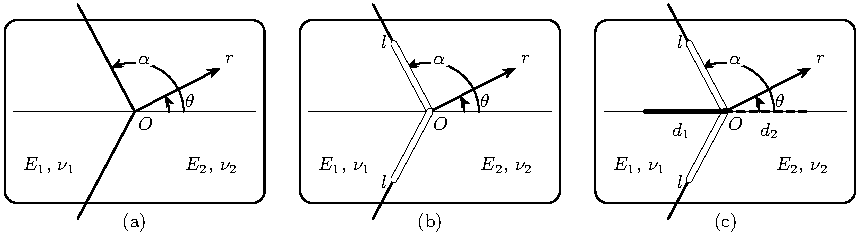
\includegraphics[width=\linewidth]{Fig1.pdf}
% M0297
\caption{Локальні конфігурації поблизу кутової точки межі поділу. (a) Непошкоджена ламана межа поділу. (b) Задана стаціонарна V-подібна міжфазна тріщина зсуву з двома гілками довжини $l$ кожна (сумарна довжина гілок $2l$). (c) Зона передруйнування довжини $d_1$ в матеріалі~1 та альтернативна зона довжини $d_2$ в матеріалі~2 (штрихова лінія). Рисунок зіставляє відповідні локальні конфігурації без заданої послідовності їх виникнення.}
% M0304
\label{fig:failure-stages}
% M0305
\end{figure}

% M0307
\subsection{Локальна задача та крайові умови}
% M0308
\label{subsec:boundary-conditions}

% M0310
Нехай $L$ — характерний зовнішній розмір тіла. Припускаємо розділення масштабів
% M0312
\begin{equation*}
  d_i\ll l\ll L
\end{equation*}
% M0315
і нехтуємо тертям між берегами міжфазної тріщини. У цій квазістатичній постановці амплітуда $C$ зовнішнього поля може змінюватися, а півдовжина тріщини $l$ і, відповідно, сумарна довжина $2l$ двох гілок залишаються сталими. Зміна навантаження змінює рівноважну довжину зони $d_i$ і пов’язані з нею локальні характеристики. У локальній задачі кусково-однорідне тіло замінюємо нескінченною площиною, а дві гілки V-подібної міжфазної тріщини вважаємо напівнескінченними. Їхню скінченну довжину та прикладене навантаження враховуємо через умову зрощування асимптотик~\citep{Nayfeh1973Perturbation}. У цьому локальному наближенні відоме поле стаціонарної міжфазної тріщини задає навантаження внутрішньої задачі поблизу $O$. Зворотний вплив малої зони передруйнування на поля у вершинах гілок тріщини не визначаємо.

% M0328
Для величини поля $f$, заданої по обидва боки променя $\theta=\alpha$, стрибок на межі поділу визначаємо за формулою
% M0330
\begin{equation*}
  \jump{f}
  =f(r,\alpha+0)-f(r,\alpha-0),
\end{equation*}
% M0334
де $\alpha+0$ і $\alpha-0$ позначають граничні значення з боку матеріалів~1 і~2 відповідно. Крайові умови випливають із трьох окремих вимог: симетрії на бісектрисах секторів обох матеріалів, неперервності напружень на межі поділу та контакту без тертя й розкриття берегів наявної міжфазної тріщини. Записуємо їх окремо:
% M0339
\begin{equation}
\label{eq:interface-boundary-conditions}
\begin{aligned}
  &\theta\in\{0,\pi\}: &&
    \tau_{r\theta}=0,
    &&\text{(симетрія)},\\
  &\theta=\alpha: &&
    \jump{\sigma_\theta}=0,\qquad
    \jump{\tau_{r\theta}}=0,
    &&\text{(неперервність напружень)},\\
  &\theta=\alpha: &&
    \tau_{r\theta}=0,\qquad
    \jump{u_\theta}=0,
    &&\text{(контакт без тертя й розкриття берегів)}.
\end{aligned}
\end{equation}
% M0355
Дві умови на дотичне напруження при $\theta=\alpha$ мають різний зміст. Умова $\jump{\tau_{r\theta}}=0$ встановлює рівність двох граничних дотичних напружень, а умова $\tau_{r\theta}=0$ — нульове спільне значення, оскільки береги тріщини контактують без тертя. Умова $\jump{u_\theta}=0$ унеможливлює нормальне розкриття берегів.

% M0361
Нехай $j=3-i$ позначає інший матеріал. На активній бісектрисі $\theta=\beta_i$ ділянка зони передруйнування $0<r<d_i$ має задані напруження, а її продовження попереду зони залишається замкненим за симетрією. Неактивна бісектриса $\theta=\beta_j$ залишається лінією симетрії для всіх $r>0$:
% M0366
\begin{equation}
\label{eq:process-zone-boundary-conditions}
\begin{aligned}
  &\theta=\beta_i: &&
  \begin{cases}
    \sigma_\theta(r,\beta_i)=\sigma_i, & 0<r<d_i,\\
    u_\theta(r,\beta_i)=0, & r>d_i,
  \end{cases}\\[4pt]
  &\theta=\beta_j,\quad j\ne i: &&
    u_\theta(r,\beta_j)=0,\qquad r>0.
\end{aligned}
\end{equation}
% M0378
Отже, задане когезійне напруження $\sigma_i$ замінює умову симетрії лише на ділянці зони передруйнування. На бісектрисі іншого матеріалу крайові умови залишаються без змін.

% M0382
На проміжних відстанях $d_i\ll r\ll l$ розв’язок має зрощуватися з асимптотичним полем міжфазної тріщини за відсутності зони передруйнування~\citep{NazarenkoKipnis2022Stress}. У внутрішній задачі умова зрощування має вигляд
% M0386
\begin{equation}
\label{eq:matched-far-field}
  \sigma_\theta(r,\beta_i)
    =CQ_i r^\lambda+o\!\left(r^{-1}\right),
    \qquad r\to\infty.
\end{equation}
% M0392
Тут $Q_i$ — амплітудний коефіцієнт для матеріалу~$i$, який залежить від кута межі поділу, пружних властивостей і довжини гілки $l$, як зазначено в \AsymptoticsAppendix. Показник $\lambda\in(-1,0)$ характеризує сингулярність кутової точки в конфігурації із заданою стаціонарною V-подібною міжфазною тріщиною. Це найменший дійсний корінь рівняння $D(-1-\lambda)=0$ в інтервалі $(-1,0)$, неперервно пов’язаний із фізичною гілкою, де $D$ — характеристичний визначник для конфігурації з тріщиною. Вирази для $D$ й $Q_i$ наведено в \AsymptoticsAppendix. Границю $r\to\infty$ розуміємо у внутрішньому масштабі зрощування асимптотик. Вона не описує далеке поле скінченного тіла. Залишковий член $o(r^{-1})$ виражає прийняту умову спадання поправки після виділення провідного сингулярного члена зовнішнього поля. Із цієї умови не робимо висновку про наступний член повного зовнішнього розкладу. Цього вибору достатньо для аналітичності введеної нижче зовнішньої трансформанти Мелліна при $\operatorname{Re}p<0$ (слабшої оцінки $O(r^{-1})$ вже було б достатньо у відкритій півплощині).

% M0409
Для подальшої побудови розв’язку методом Вінера--Гопфа використовуємо принцип суперпозиції, як і в спорідненій задачі~\citep{KaminskyDudykPolishchuk2024}. Віднімаємо відоме поле стаціонарної V-подібної міжфазної тріщини без зони передруйнування та вводимо коригувальне нормальне напруження
% M0412
\begin{equation*}
  \widehat{\sigma}_i(r)
  =\sigma_\theta(r,\beta_i)-CQ_i r^\lambda.
\end{equation*}
% M0416
З умови зрощування тоді випливає
% M0417
\begin{equation*}
  \widehat{\sigma}_i(r)=o(r^{-1}),
  \qquad r\to\infty,
\end{equation*}
% M0421
а на ділянці зони передруйнування $0<r<d_i$ маємо
% M0422
\begin{equation*}
  \widehat{\sigma}_i(r)
  =\sigma_i-CQ_i r^\lambda.
\end{equation*}
% M0426
Поле стаціонарної V-подібної тріщини без зони передруйнування задовольняє умову симетрії на бісектрисі $u_\theta=0$, тому його віднімання не змінює трансформанти градієнта переміщення, використаної нижче. Отже, функціональну задачу формулюємо для коригувального поля, включивши відомий степеневий член до заданої частини.

% M0431
Зона передруйнування може утворитися в матеріалі~$i$ лише тоді, коли нормальне напруження на його бісектрисі є розтягувальним. Із формули~\eqref{eq:matched-far-field} випливає умова фізичної допустимості
% M0434
\begin{equation*}
  CQ_i>0.
\end{equation*}
% M0437
Отже, модель вимагає виконання $Cg_2<0$ для контакту між берегами міжфазної тріщини та $CQ_i>0$ для утворення зони передруйнування в матеріалі~$i$. Ці умови допустимості перевіряємо незалежно для обох матеріалів. Ані в базових розрахунках, ані під час ширшого перебору параметрів, описаного в розділі~\ref{sec:numerical-results}, не виявлено випадку, коли обидва матеріали допустимі одночасно. Це спостереження отримано в результаті числового аналізу в дослідженій області параметрів, і його не поширюємо як загальну теорему єдиності.

% M0446
\subsection{Асимптотичні поля поблизу вершини зони передруйнування}
% M0447
\label{subsec:zone-tip-asymptotics}

% M0449
Поблизу зовнішньої вершини лінії розриву переміщення напруження й градієнт нормального переміщення мають стандартну для однорідного матеріалу асимптотику типу оберненого квадратного кореня. Хоча тіло складається з двох матеріалів, точка $r=d_i>0$ лежить усередині матеріалу $i$ поза кутовою точкою межі поділу. Тому провідний член поля у вершині має стандартний вигляд поля моди~I в однорідному матеріалі:
% M0455
\begin{equation}
\label{eq:zone-tip-asymptotics}
\begin{aligned}
  &\theta=\beta_i,\quad r\to d_i+0:
  &&\sigma_\theta(r,\beta_i)
    \sim \frac{k_i}{\sqrt{2\pi(r-d_i)}},\\[3pt]
  &\theta=\beta_i,\quad r\to d_i-0:
  &&\frac{\partial u_\theta}{\partial r}(r,\beta_i)
    \sim -\frac{2(1-\nu_i^2)}{E_i}
    \frac{k_i}{\sqrt{2\pi(d_i-r)}}.
\end{aligned}
\end{equation}
% M0467
Тут $k_i$ — локальний коефіцієнт інтенсивності напружень за модою~I у вершині зони передруйнування. Позначення $r\to d_i+0$ й $r\to d_i-0$ відповідають наближенню до вершини з ділянки попереду зони та зсередини зони відповідно. Крайову задачу замикаємо стандартною для цієї моделі умовою регулярності напружень~\citep{KaminskyDudykPolishchuk2024},
% M0472
\begin{equation*}
  k_i=0.
\end{equation*}
% M0475
За заданого $d_i$ розв’язок трансформованої крайової задачі загалом дає ненульовий коефіцієнт $k_i$. Кінцева точка $d_i$ сама є невідомою, тому маємо однопараметричну задачу з вільною межею. Єдина скалярна умова регулярності $k_i=0$ є відповідною умовою розв’язності й визначає рівноважне значення $d_i$. Вона усуває лише сингулярний член типу оберненого квадратного кореня й не вимагає, щоб обмежена частина напруження у вершині зони дорівнювала нулю.

% M0484
\section{Визначення рівноважних параметрів зони передруйнування}
% M0485
\label{sec:derivation}

% M0487
\subsection{Перетворення Мелліна та функціональне рівняння}
% M0488
\label{subsec:mellin}

% M0490
Для розв’язання локальної задачі вводимо безрозмірну радіальну координату
% M0491
\begin{equation*}
  \rho=\frac{r}{d_i}
\end{equation*}
% M0494
й застосовуємо інтегральне перетворення Мелліна до крайової задачі \eqref{eq:interface-boundary-conditions}--\eqref{eq:matched-far-field}. Нехай $p$ — комплексна змінна перетворення Мелліна. У трансформанті переміщення $\partial u_\theta/\partial r$ розуміємо як значення переміщення на березі, додатне в напрямку розкриття, відповідно до розділу~\ref{subsec:geometry}. Трансформанти коригувального нормального напруження поза зоною та градієнта нормального переміщення всередині зони визначаємо так:
% M0501
\begin{equation*}
\begin{aligned}
  \Phi_i^+(p)
    &=\int_1^\infty
      \widehat{\sigma}_i(\rho d_i)\rho^p\,\dd\rho,\\
  \Phi_i^-(p)
    &=\frac{E_i}{2(1-\nu_i^2)}
      \int_0^1
      \left.
      \frac{\partial u_\theta}{\partial r}
      \right|_{\substack{r=\rho d_i\\\theta=\beta_i}}
      \rho^p\,\dd\rho.
\end{aligned}
\end{equation*}
% M0515
Оскільки $\widehat{\sigma}_i(r)=o(r^{-1})$ за $r\to\infty$, інтеграл для $\Phi_i^+$ задає аналітичну функцію при $\operatorname{Re}p<0$. У вужчій області $\operatorname{Re}p<-1-\lambda$, де збігається також трансформанта повного напруження до віднімання зовнішнього поля,
% M0519
\begin{equation*}
  \widetilde{\Phi}_i^+(p)
  =\int_1^\infty
    \sigma_\theta(\rho d_i,\beta_i)\rho^p\,\dd\rho
\end{equation*}
% M0524
обидві функції задовольняють співвідношення
% M0525
\begin{equation*}
  \Phi_i^+(p)
  =\widetilde{\Phi}_i^+(p)
   +\frac{CQ_i d_i^\lambda}{p+\lambda+1},
\end{equation*}
% M0530
що усуває полюс, породжений зрощеним зовнішнім полем. Поблизу кутової точки градієнт переміщення має порядок $r^{\lambda_i}$, тому $\Phi_i^-$ аналітична при $\operatorname{Re}p>-1-\lambda_i$. Верхні індекси в $\Phi_i^+$ й $\Phi_i^-$ позначають функції, віднесені відповідно до лівої і правої півплощин, і не вказують знака фізичної величини.

% M0536
На активній ділянці $0<\rho<1$ коригувальне напруження дорівнює $\sigma_i-CQ_i d_i^\lambda\rho^\lambda$, звідки
% M0538
\begin{equation*}
  \int_0^1
  \left(\sigma_i-CQ_i d_i^\lambda\rho^\lambda\right)
  \rho^p\,\dd\rho
  =
  \frac{\sigma_i}{p+1}
  -\frac{CQ_i d_i^\lambda}{p+\lambda+1}.
\end{equation*}
% M0546
Для повноти наведемо схему виключення невідомих, що приводить до скалярного функціонального рівняння. Для компоненти Мелліна функція напружень Ері вигляду $r^{1-p}f(\theta)$ задовольняє співвідношення
% M0549
\begin{equation*}
  \left[\frac{\dd^2}{\dd\theta^2}+(1-p)^2\right]
  \left[\frac{\dd^2}{\dd\theta^2}+(1+p)^2\right]f=0.
\end{equation*}
% M0553
У кожному секторі чотири кутові коефіцієнти визначаються умовою нульового дотичного напруження на бісектрисі сектора та нормальним і дотичним напруженнями на межі поділу. Умова нульового градієнта нормального переміщення на неактивній бісектрисі разом з умовами неперервності нормального переміщення та напружень при $\theta=\alpha$ дає змогу виключити амплітуди на межі поділу. Отримане співвідношення між трансформантою напруження на активній бісектрисі $T_i(p)$ і трансформантою градієнта переміщення, додатного в напрямку розкриття, має вигляд
% M0560
\begin{equation*}
  T_i(p)=-\frac{D_i(p)}{D(p)}\,\Phi_i^-(p).
\end{equation*}
% M0563
Тут $D(p)$ — визначник задачі для кутової точки зі стаціонарною тріщиною, а $D_i(p)$ — визначник, отриманий за умови, що на активній бісектрисі допускається розрив нормального переміщення. Їх явні вирази наведено нижче та в додатку~\ref{app:asymptotics}. Оскільки
% M0567
\begin{equation*}
  \frac{D_i(p)}{D(p)}=\tan(\pi p)\,G_i(p)
\end{equation*}
% M0570
і
% M0571
\begin{equation*}
  T_i(p)=
  \Phi_i^+(p)+\frac{\sigma_i}{p+1}
  -\frac{CQ_i d_i^\lambda}{p+\lambda+1},
\end{equation*}
% M0576
отримуємо функціональне рівняння
% M0577
\begin{equation}
\label{eq:wiener-hopf-functional}
  \Phi_i^+(p)
  +\frac{\sigma_i}{p+1}
  -\frac{CQ_i d_i^\lambda}{p+\lambda+1}
  =-\tan(\pi p)G_i(p)\Phi_i^-(p),
\end{equation}
% M0584
яке спочатку справджується в спільній смузі збіжності
% M0585
\begin{equation*}
  \max\{-1-\lambda,-1-\lambda_i\}
  <\operatorname{Re}p<0.
\end{equation*}
% M0589
Тут $\operatorname{Re}p$ позначає дійсну частину $p$. У цій смузі обидві частини виражають одне й те саме аналітичне співвідношення. Далі функціональне рівняння дає аналітичне (або, за наявності явних раціональних членів, мероморфне) продовження комбінацій, потрібних для факторизації, на контур $\operatorname{Re}p=0$. Для цього продовження збіжність самого інтеграла, що визначає $\Phi_i^+$, на уявній осі не потрібна. Ядро $G_i(p)$ має вигляд
% M0596
\begin{equation*}
  G_i(p)=\frac{D_i(p)\cos(\pi p)}{D(p)\sin(\pi p)}.
\end{equation*}
% M0599
Тут $D(p)$ — характеристичний визначник для кутової точки із заданою стаціонарною V-подібною міжфазною тріщиною зсуву, наведений у додатку~\ref{app:asymptotics}. Для плоскої деформації визначаємо безрозмірне відношення пружних характеристик $e$ і параметри матеріалів $\kappa_i$ за формулами
% M0604
\begin{equation*}
  e=\frac{1+\nu_2}{1+\nu_1}\frac{E_1}{E_2},
  \qquad
  \kappa_i=3-4\nu_i.
\end{equation*}
% M0609
Характеристичні визначники $D_1(p)$ і $D_2(p)$ для конфігурацій із зоною передруйнування в матеріалах~1 і~2 відповідно мають вигляд
% M0611
\begin{equation*}
\begin{aligned}
  D_1(p)={}&2e(1+\kappa_2)
    [\cos(2p\alpha)-\cos(2\alpha)]
    \{\sin^2[p(\pi-\alpha)]-p^2\sin^2\alpha\}\\
  &+(1+\kappa_1)
    [\sin(2p\alpha)+p\sin(2\alpha)]
    [\sin(2p(\pi-\alpha))-p\sin(2\alpha)],\\[2pt]
  D_2(p)={}&2(1+\kappa_1)
    [\cos(2p(\pi-\alpha))-\cos(2\alpha)]
    [\sin^2(p\alpha)-p^2\sin^2\alpha]\\
  &+e(1+\kappa_2)
    [\sin(2p(\pi-\alpha))-p\sin(2\alpha)]
    [\sin(2p\alpha)+p\sin(2\alpha)].
\end{aligned}
\end{equation*}
% M0627
Зокрема, показник сингулярності $\lambda_i$ у кутовій точці за наявності зони в матеріалі~$i$ визначаємо з рівняння
% M0629
\begin{equation*}
  D_i(-1-\lambda_i)=0,
\end{equation*}
% M0632
де $\lambda_i$ — найменший дійсний корінь в інтервалі $(-1,0)$, неперервно пов’язаний із відповідною фізичною гілкою. Як і раніше, $\alpha=\pi/2$ розглядаємо лише як вироджений граничний випадок.

% M0636
\subsection{Факторизація Вінера--Гопфа}
% M0637
\label{subsec:wiener-hopf}

% M0639
Рівняння~\eqref{eq:wiener-hopf-functional} розв’язуємо методом Вінера--Гопфа~\citep{noble1958wienerhopf} за підходом, використаним у спорідненій крайовій задачі~\citep{KaminskyDudykPolishchuk2024}. Множники $G_i^\pm(p)$ визначаємо інтегралом Коші
% M0643
\begin{equation*}
  \exp\left\{
    \frac{1}{2\pi\ii}
    \int_{-\ii\infty}^{\ii\infty}
      \frac{\log G_i(z)}{z-p}\,\dd z
  \right\}
  =
  \begin{cases}
    G_i^+(p), & \operatorname{Re}p<0,\\
    G_i^-(p), & \operatorname{Re}p>0,
  \end{cases}
\end{equation*}
% M0655
де $z$ — комплексна змінна інтегрування та $\ii^2=-1$. Контур спрямовано вгору вздовж уявної осі. Множники на нескінченності нормовано умовою $G_i^\pm(p)\to1$. За допомогою інтеграла Коші факторизуємо додатний граничний символ $G_i(\ii t)$ з нульовим індексом на уявній осі. За цієї орієнтації контуру співвідношення Сохоцького--Племеля для стрибка дає факторизацію у вигляді \emph{відношення} множників
% M0661
\begin{equation*}
  G_i(\ii t)=
  \frac{G_i^+(\ii t)}{G_i^-(\ii t)}.
\end{equation*}
% M0665
Для використаного тут парного ядра зі співвідношення симетрії маємо
% M0666
\begin{equation}
\label{eq:factor-reflection}
  G_i^-(p)=\frac{1}{G_i^+(-p)}
\end{equation}
% M0670
у відповідних точках двох півплощин. Зокрема, односторонні границі в усувній особливій точці $p=0$ задовольняють умову
% M0672
\begin{equation}
\label{eq:factor-zero}
  G_i^+(0)=\sqrt{G_i(0)},\qquad
  G_i^-(0)=\frac{1}{\sqrt{G_i(0)}}.
\end{equation}
% M0677
Мероморфне продовження $G_i(p)$ має полюси й нулі поза контуром факторизації, пов’язані з характеристичними визначниками. Вони не створюють особливих точок окремого множника Коші в точках обчислення $-1$ та $-1-\lambda$ у лівій півплощині. Значення $G_i^+(-1)$ й $G_i^+(-1-\lambda)$ є звичайними значеннями множника, визначеного за граничним символом.

% M0684
Введемо також допоміжні гамма-функціональні множники
% M0685
\begin{equation*}
  K^\pm(p)=
  \frac{\Gamma(1\mp p)}{\Gamma(\tfrac12\mp p)}.
\end{equation*}
% M0689
Із формул доповнення Ейлера випливає тотожність
% M0690
\begin{equation}
\label{eq:gamma-factor-identity}
  K^+(p)K^-(p)=p\cot(\pi p),
\end{equation}
% M0694
яка явно виділяє елементарний тригонометричний множник.

% M0696
Щоб показати розділення за методом Вінера--Гопфа, покладемо
% M0697
\begin{equation*}
  a=1+\lambda,\qquad
  P=CQ_i d_i^\lambda,\qquad
  L(p)=\frac{K^+(p)}{pG_i^+(p)}.
\end{equation*}
% M0702
Помноживши рівняння~\eqref{eq:wiener-hopf-functional} на $L(p)$ і використавши рівняння~\eqref{eq:gamma-factor-identity}, отримуємо
% M0704
\begin{equation*}
\begin{aligned}
  &L\Phi_i^+
  +\sigma_i\frac{L(p)-L(-1)}{p+1}
  -P\frac{L(p)-L(-a)}{p+a}\\
  &\qquad=
  -\frac{\Phi_i^-}{K^-(p)G_i^-(p)}
  -\frac{\sigma_iL(-1)}{p+1}
  +\frac{PL(-a)}{p+a}.
\end{aligned}
\end{equation*}
% M0715
Віднімання усувають позірні полюси неоднорідної частини з лівої аналітичної частини. Решта полюсів неоднорідної частини лежать поза правою півплощиною. Отже, обидві частини задають спільне аналітичне продовження через контур факторизації. Оцінки поблизу кінцевих точок забезпечують прямування цього продовження до нуля на нескінченності. За теоремою Ліувілля воно тотожно дорівнює нулю. Розв’язуючи отримані співвідношення для лівої та правої частин, знаходимо
% M0721
\begin{equation}
\label{eq:wiener-hopf-solution}
\begin{aligned}
  \Phi_i^+(p)={}&
  -\frac{pG_i^+(p)}{K^+(p)}
  \Bigg\{
    \frac{\sigma_i}{p+1}
    \left[
      \frac{K^+(p)}{pG_i^+(p)}
      +\frac{K^+(-1)}{G_i^+(-1)}
    \right]\\
  &\hspace{37mm}
    -\frac{CQ_i d_i^\lambda}{p+\lambda+1}
    \left[
      \frac{K^+(p)}{pG_i^+(p)}
      +\frac{K^+(-\lambda-1)}
      {(\lambda+1)G_i^+(-\lambda-1)}
    \right]
  \Bigg\},\\[-1pt]
  &\hspace{8mm}\operatorname{Re}p<0,\\[3pt]
  \Phi_i^-(p)={}&
  K^-(p)G_i^-(p)
  \Bigg\{
    \frac{\sigma_iK^+(-1)}{(p+1)G_i^+(-1)}
    -\frac{CQ_i d_i^\lambda K^+(-\lambda-1)}
    {(\lambda+1)(p+\lambda+1)G_i^+(-\lambda-1)}
  \Bigg\},\\[-1pt]
  &\hspace{8mm}\operatorname{Re}p>0.
\end{aligned}
\end{equation}
% M0751
Для розглянутих тут ядер числові перевірки показують, що $G_i(\ii t)$ є дійсною, додатною й парною функцією дійсної змінної $t$ та прямує до одиниці за $|t|\to\infty$. Тому для дійсного $p<0$ плюс-фактор можна обчислити чисельно за допомогою дійсного інтеграла
% M0756
\begin{equation*}
  \log G_i^+(p)
  =-\frac{p}{\pi}\int_0^\infty
    \frac{\log G_i(\ii t)}{t^2+p^2}\,\dd t,
  \qquad p<0.
\end{equation*}
% M0762
У числових розрахунках перевіряємо, що ядро є дійсним і додатним на контурі факторизації та наближається до одиниці за великих $|t|$.

% M0766
\subsection{Довжина зони передруйнування}
% M0767
\label{subsec:zone-length}

% M0769
За $p\to+\infty$ з другого співвідношення рівняння~\eqref{eq:wiener-hopf-solution} маємо
% M0771
\begin{equation*}
  \Phi_i^-(p)\sim\frac{1}{\sqrt{p}}
  \left[
    \frac{\sigma_iK^+(-1)}{G_i^+(-1)}
    -\frac{CQ_i d_i^\lambda K^+(-\lambda-1)}
    {(\lambda+1)G_i^+(-\lambda-1)}
  \right].
\end{equation*}
% M0779
Застосування теореми абелевого типу~\citep{noble1958wienerhopf} до асимптотики у вершині~\eqref{eq:zone-tip-asymptotics} також дає
% M0781
\begin{equation*}
  \Phi_i^-(p)\sim-\frac{k_i}{\sqrt{2pd_i}}.
\end{equation*}
% M0784
Порівняння цих виразів дає локальний коефіцієнт інтенсивності напружень
% M0785
\begin{equation*}
  k_i=-\sqrt{2d_i}
  \left[
    \frac{\sigma_iK^+(-1)}{G_i^+(-1)}
    -\frac{CQ_i d_i^\lambda K^+(-\lambda-1)}
    {(\lambda+1)G_i^+(-\lambda-1)}
  \right].
\end{equation*}
% M0793
Умова $k_i=0$, що усуває сингулярний член типу оберненого квадратного кореня з прийнятої асимптотики у вершині, визначає довжину зони:
% M0795
\begin{equation}
\label{eq:process-zone-length}
  d_i=
  \left[
    \frac{CQ_iK^+(-\lambda-1)G_i^+(-1)}
    {\sigma_i(1+\lambda)K^+(-1)G_i^+(-\lambda-1)}
  \right]^{-1/\lambda}.
\end{equation}
% M0803
Оскільки $-1<\lambda<0$, для дійсного додатного $d_i$ необхідно, щоб виконувалася умова $CQ_i>0$, що узгоджується з умовою фізичної допустимості в розділі~\ref{subsec:boundary-conditions}. За фіксованої геометрії та фіксованої довжини гілки V-подібної тріщини $l$ з формули~\eqref{eq:process-zone-length} випливає степенева залежність $d_i\propto |C|^{-1/\lambda}$. Отже, зміна величини зовнішнього навантаження $|C|$ породжує сім’ю квазістатичних рівноважних станів зони передруйнування $d_i(C)$ за сталої довжини кожної гілки V-подібної тріщини. В ідеалізованій сингулярній постановці ця залежність сама по собі не задає скінченного порога утворення зони. Для кожного ненульового фізично допустимого $C$ маємо $d_i>0$, причому $d_i\to0$ за $|C|\to0$. Скінченний поріг матеріалу вводимо на наступному етапі, визначаючи ініціювання відгалуження за критичною характеристикою рівноважної зони.

% M0818
За фіксованої геометрії, довжини гілки V-подібної тріщини $l$, пружних властивостей і прикладеного навантаження з тієї самої формули випливає залежність від нормального когезійного напруження:
% M0821
\begin{equation*}
  d_i\propto \sigma_i^{1/\lambda}
  =\sigma_i^{-1/|\lambda|}.
\end{equation*}
% M0825
Оскільки $-1<\lambda<0$, зі зменшенням $\sigma_i$ довжина зони передруйнування збільшується.

% M0828
Використовуючи співвідношення
% M0829
\begin{equation*}
  Q_i=g_1q_i l^{\lambda_0-\lambda},
\end{equation*}
% M0832
де $g_1$ — кутовий коефіцієнт для непошкодженої кутової точки, а $q_i$ — безрозмірний амплітудний коефіцієнт, обидва наведені в додатку~\ref{app:asymptotics}, із формули~\eqref{eq:process-zone-length} отримуємо
% M0836
\begin{equation}
\label{eq:normalized-process-zone-length}
  \frac{d_i}{l}=
  \left[
    \frac{Cl^{\lambda_0}}{\sigma_i}
    \frac{g_1q_iK^+(-1-\lambda)G_i^+(-1)}
    {(1+\lambda)K^+(-1)G_i^+(-1-\lambda)}
  \right]^{-1/\lambda}.
\end{equation}
% M0845
Це співвідношення також дає змогу перевірити маломасштабне припущення $d_i/l\ll1$, прийняте в локальній постановці.

% M0848
\subsection{Розкриття й енергетичний параметр}
% M0849
\label{subsec:zone-parameters}

% M0851
Нехай розкриття зони передруйнування в кутовій точці дорівнює $\delta_i=\jump{u_\theta(0,\beta_i)}$, де стрибок між двома берегами зони взято в заданому вище додатному напрямку розкриття. Із визначення $\Phi_i^-(p)$ випливає
% M0855
\begin{equation*}
  \delta_i
  =-2
    \left.
      \left(\frac{\partial u_\theta}{\partial r}\right)^*
    \right|_{p=0,\,\theta=\beta_i}
  =-\frac{4(1-\nu_i^2)d_i}{E_i}\Phi_i^-(0).
\end{equation*}
% M0863
Тут зірочка позначає розмірний момент трансформанти. Для $f(r)=\partial u_\theta(r,\beta_i)/\partial r$ маємо $f^*(p)=\int_0^{d_i}f(r)(r/d_i)^p\,\dd r$. Множник два враховує симетричні переміщення обох берегів зони.

% M0869
Два моменти трансформанти, що входять до виразів для розкриття й роботи, можна обчислити безпосередньо. Визначимо
% M0871
\begin{equation*}
  A_i=\frac{\sigma_iK^+(-1)}{G_i^+(-1)}.
\end{equation*}
% M0874
Після накладання умови регулярності $k_i=0$ рівняння~\eqref{eq:wiener-hopf-solution} набуває вигляду
% M0876
\begin{equation}
\label{eq:phi-minus-regular}
  \Phi_i^-(p)=
  \frac{\lambda A_i K^-(p)G_i^-(p)}
  {(p+1)(p+1+\lambda)}.
\end{equation}
% M0882
Використовуючи формули~\eqref{eq:factor-reflection}--\eqref{eq:factor-zero}, отримуємо
% M0883
\begin{equation*}
  K^-(0)=\frac{1}{\sqrt{\pi}},\qquad
  G_i^-(0)=\frac{1}{\sqrt{G_i(0)}},
\end{equation*}
% M0887
звідки
% M0888
\begin{equation}
\label{eq:phi-minus-zero}
  \Phi_i^-(0)=
  \frac{\sigma_i\lambda K^+(-1)}
  {(1+\lambda)G_i^+(-1)\sqrt{\pi G_i(0)}}.
\end{equation}
% M0894
Аналогічно маємо
% M0895
\begin{equation*}
  K^-(1)=K^+(-1)=\frac{2}{\sqrt{\pi}},\qquad
  G_i^-(1)=\frac{1}{G_i^+(-1)},
\end{equation*}
% M0899
і тому
% M0900
\begin{equation}
\label{eq:phi-minus-one}
  \Phi_i^-(1)=
  \frac{2\lambda\sigma_i}
  {\pi(\lambda+2)[G_i^+(-1)]^2}.
\end{equation}
% M0906
Формула~\eqref{eq:phi-minus-zero} явно показує, що за прийнятої факторизації у вигляді відношення множників $\sqrt{G_i(0)}$ стоїть у знаменнику. Підставляючи цей вираз у визначення розкриття, отримуємо
% M0909
\begin{equation}
\label{eq:process-zone-opening}
  \delta_i=
  -\frac{4(1-\nu_i^2)\sigma_i\lambda K^+(-1)}
  {E_i\sqrt{\pi G_i(0)}(1+\lambda)G_i^+(-1)}d_i.
\end{equation}
% M0915
За фіксованих властивостей матеріалів і геометрії коефіцієнт при $d_i$ у формулі~\eqref{eq:process-zone-opening} сталий. Тому зі зміною прикладеного навантаження розкриття пропорційне довжині зони: $\delta_i\propto d_i$. Якщо прикладене навантаження зафіксувати й змінювати $\sigma_i$, з попередньої степеневої залежності випливає
% M0920
\begin{equation*}
  \delta_i\propto \sigma_i d_i
  \propto \sigma_i^{1+1/\lambda}
  =\sigma_i^{1-1/|\lambda|}.
\end{equation*}
% M0925
Показник $1-1/|\lambda|$ від’ємний. Тому зі зменшенням опору відриву збільшуються і довжина зони, і її розкриття.

% M0928
У прийнятій моделі роботу $W_i$ сил опору відриву на одиницю товщини в напрямку, перпендикулярному до площини задачі, визначаємо за формулою~\citep{Cherepanov1986}
% M0931
\begin{equation*}
  W_i=\sigma_i\int_0^{d_i}
      \jump{u_\theta(r,\beta_i)}\,\dd r
  =-\frac{4(1-\nu_i^2)\sigma_i}{E_i}d_i^2\Phi_i^-(1).
\end{equation*}
% M0936
За формулою~\eqref{eq:phi-minus-one} отримуємо
% M0937
\begin{equation*}
  W_i=-\frac{8\lambda(1-\nu_i^2)\sigma_i^2}
  {\pi(\lambda+2)[G_i^+(-1)]^2E_i}d_i^2.
\end{equation*}
% M0941
Диференціювання роботи за довжиною зони вздовж сім’ї рівноважних станів за фіксованої геометрії та властивостей матеріалів визначає зональний енергетичний параметр $J_i$:
% M0944
\begin{equation}
\label{eq:process-zone-energy-parameter}
  J_i=\frac{\dd W_i}{\dd d_i}
  =-\frac{16\lambda(1-\nu_i^2)\sigma_i^2}
  {\pi(\lambda+2)[G_i^+(-1)]^2E_i}d_i.
\end{equation}
% M0950
Для числового аналізу введемо безрозмірні параметри навантаження, розкриття й енергії $\sigmap$, $\delta_i'$ та $J_i'$ відповідно:
% M0953
\begin{equation*}
  \sigmap=\frac{Cl^{\lambda_0}}{\sigma_i},
  \qquad
  \delta_i'=\frac{E_i\delta_i}
  {4(1-\nu_i^2)\sigma_i l},
  \qquad
  J_i'=\frac{E_iJ_i}
  {4(1-\nu_i^2)\sigma_i^2l}.
\end{equation*}
% M0962
Штрихи тут позначають нормування, а не диференціювання. Тоді формули~\eqref{eq:normalized-process-zone-length}, \eqref{eq:process-zone-opening} й \eqref{eq:process-zone-energy-parameter} набувають вигляду
% M0966
\begin{equation*}
\begin{aligned}
  \frac{d_i}{l}
    &=\left[
      \sigmap\,
      \frac{g_1q_iK^+(-1-\lambda)G_i^+(-1)}
      {(1+\lambda)K^+(-1)G_i^+(-1-\lambda)}
    \right]^{-1/\lambda},\\[2pt]
  \delta_i'
    &=-\frac{\lambda K^+(-1)}
      {\sqrt{\pi G_i(0)}(1+\lambda)G_i^+(-1)}
      \frac{d_i}{l},\\[2pt]
  J_i'
    &=-\frac{4\lambda}
      {\pi(\lambda+2)[G_i^+(-1)]^2}
      \frac{d_i}{l}.
\end{aligned}
\end{equation*}
% M0984
У всіх трьох співвідношеннях використано показник $\lambda$ у кутовій точці заданої стаціонарної V-подібної міжфазної тріщини зсуву, тобто корінь рівняння $D(-1-\lambda)=0$. Показники $\lambda_1$ та $\lambda_2$ описують сингулярність кутової точки за наявності зони й не замінюють $\lambda$ у формулах для параметрів зони.

% M0991
За фіксованих геометрії та властивостей матеріалів $\delta_i$ і $J_i$ лінійно залежать від тієї самої рівноважної довжини зони $d_i$. Виключаючи $d_i$ з формул~\eqref{eq:process-zone-opening} і~\eqref{eq:process-zone-energy-parameter}, отримуємо
% M0995
\begin{equation}
\label{eq:energy-opening-relation}
  J_i=\chi_i\sigma_i\delta_i,
  \qquad
  \chi_i=
  \frac{4(1+\lambda)\sqrt{\pi G_i(0)}}
  {\pi(\lambda+2)G_i^+(-1)K^+(-1)}.
\end{equation}
% M1003
Тут $\chi_i$ — безрозмірний коефіцієнт пропорційності, що визначається локальною геометрією та пружним контрастом.

% M1006
У прийнятій локальній моделі $J_i$ має зміст зонального енергетичного параметра. Незалежного виведення глобального контурного інтеграла тут не проводимо. За аналогією з критеріями, що використовують зону передруйнування для відхилення міжфазної тріщини~\citep{KaminskyEtAl2023}, ініціювання відгалуження можна описати енергетичним критерієм
% M1011
\begin{equation*}
  J_i=J_{i\mathrm{c}},
\end{equation*}
% M1014
де $J_{i\mathrm{c}}$ — критична характеристика, яку в межах цього критерію задають незалежно. Як альтернативу можна використати деформаційний критерій
% M1016
\begin{equation*}
  \delta_i=\delta_{i\mathrm{c}}
\end{equation*}
% M1019
у якому $\delta_{i\mathrm{c}}$ задають незалежно як критичне розкриття. За фіксованих геометрії та властивостей матеріалів із формули~\eqref{eq:energy-opening-relation} випливає, що обидва критерії описують ту саму однопараметричну сім’ю локальних станів і визначають той самий критичний стан лише за узгодженого калібрування незалежно заданих критичних параметрів:
% M1025
\begin{equation*}
  J_{i\mathrm{c}}
  =\chi_i\sigma_i\delta_{i\mathrm{c}}.
\end{equation*}
